\documentclass[a4paper,11pt]{article}

\usepackage{pos}
% \usepackage{ulem}
\usepackage{cancel}
\usepackage{pgfplots}
\usepackage{wrapfig}
\usepackage{subcaption}
\usepackage{mathtools}
\pgfplotsset{compat=1.18}

\title{HMC with Normalizing Flows}
%% \ShortTitle{Short Title for header}

% TODO: Add citations !!

\author*[a]{Sam Foreman}
\author[b, c]{Taku Izubuchi}
\author[d]{Luchang Jin}
\author[a]{Xiao-Yong Jin}
\author[a]{James C. Osborn}
\author[b]{Akio Tomiya}

\affiliation[a]{Argonne National Laboratory,\\
  Lemont, IL 60439}

\affiliation[b]{RIKEN,\\
 2-1 Hirosawa, Wako, Saitama, 351-0198, Japan}

\affiliation[c]{Brookhaven National Laboratory,\\
 Upton, NY 11973}

\affiliation[d]{Dept. of Physics, University of Connecticut,\\
 Storrs, CT 06269}

\emailAdd{foremans@anl.gov}
\emailAdd{izubuchi@bnl.gov}
\emailAdd{luchang.jin@uconn.edu}
\emailAdd{xjin@anl.gov}
\emailAdd{osborn@alcf.anl.gov}

\abstract{%
    We propose using Normalizing Flows as a trainable kernel within the
    molecular dynamics update of Hamiltonian Monte Carlo (HMC).
    %
    By learning (invertible) transformations that simplify our dynamics, we can
    outperform traditional methods at generating independent configurations.
    %
    We show that, using a carefully constructed network architecture, our
    approach can be easily scaled to large lattice volumes with minimal
    retraining effort.
}

\FullConference{%
  % *** FIXME: Name of conference, ***\\
  % *** FIXME: day-day Month YEAR ***\\
  % *** FIXME: Location, City, Country ***
  The 38th International Symposium on Lattice Field Theory\\
  26-30 July 2021\\
  Zoom / Gather @ MIT, Cambridge MA, USA\\
}

%% \tableofcontents

\begin{document}
\maketitle
\section{\label{sec:intro}Introduction}
For a random variable \(z\) with a given distribution \(z \sim r(z)\), and an
invertible function \(x = f(z)\) with \(z = f^{-1}(x)\), we can use the change
of variables formula to write
%
\begin{equation}
    p(x) = r(z)\left|\det\frac{\partial z}{\partial x}\right| =
    r(f^{-1}(x))\left|\det\frac{\partial f^{-1}}{\partial x}\right|
\end{equation}
%
where \(r(z)\) is the (simple) prior density, and our goal is to generate
independent samples from the (difficult) target distribution \(p(x)\).
%
This can be done using \emph{normalizing flows}~\cite{rezende2015variational}
to construct a model density \(q(x)\) that approximates the target
distribution, i.e. \(q(\cdot)\simeq p(\cdot)\) for a suitably-chosen flow
\(f\).

\begin{figure}[htpb]
    \centering
    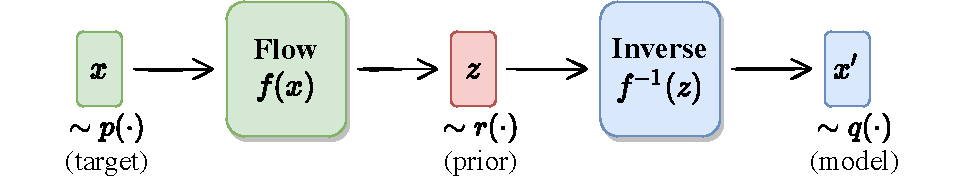
\includegraphics[width=\textwidth]{assets/flow_model.pdf}
    % 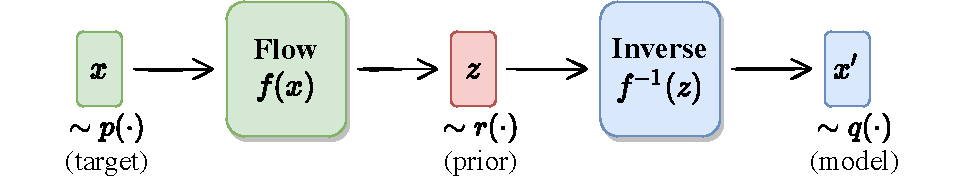
\includegraphics[width=\textwidth]{assets/flow_model.pdf}
    \caption{\label{fig:flow_model} Using a flow to generate data \(x'\). Image
    adapted from~\cite{weng2018flow}}
\end{figure}
%
We can construct a normalizing flow by composing multiple invertible functions
\(f_{i}\) so that \(x\equiv \left[f_{1}\odot f_{2}\odot \cdots \odot
f_{K}\right](z)\).
%
In practice, the functions \(f_{i}\) are usually implemented as \emph{coupling
layers}, which update an ``active'' subset of the variables, conditioned on the
complimentary ``frozen'' variables~\cite{Kanwar:2020xzo,Albergo:2021vyo}.
%
\subsection{\label{subsec:coupling_layers}Affine Coupling Layers}
A particularly useful template function for constructing our normalizing flows
is the affine coupling layer~\cite{DinhSB16,rezende2015variational},
%
\begin{align*}
    f(x_{1}, x_{2}) &= \left(e^{s(x_2)}x_{1} + t(x_{2}),\, x_{2}\right),
        \quad\text{with}\quad \log J(x) = \sum_{k}\left[s(x_{2})\right]_{k}\\
    f^{-1}(x'_{1}, x'_{2}) &= \left((x'_{1}-t(x'_{2}))e^{-s(x'_{2})},\, x'_{2}\right),
        \quad\text{with}\quad \log J(x') = \sum_{k}-\left[s(x'_{2})\right]_{k}
\end{align*}
%
where \(s(x_{2})\) and \(t(x_{2})\) are of the same dimensionality as \(x_{1}\)
and the functions act element-wise on the inputs.

In order to effectively draw samples from the correct target distribution
\(p(\cdot)\), our goal is to minimize the error introduced by approximating
\(q(\cdot)\simeq p(\cdot)\).
%
To do so, we use the (reverse) Kullback-Leibler (KL) divergence from
Eq.~\ref{eq:kl_div}, which is minimized when \(p=q\).
%
\begin{align}
    \label{eq:kl_div}
    D_{\mathrm{KL}}(q\|p) 
    &\equiv\int dy q(y)\left[\log q(y) - \log p(y)\right]\\
    &\simeq \frac{1}{N}\sum_{i=1}^{N} \left[\log q(y_{i})-\log p(y_{i})\right],
        \,\,\text{where}\,\, y_{i}\sim q
\end{align}
%
\section{\label{sec:trivializing_map}Trivializing Map}
%
Our goal is to evaluate expectation values of the form
%
\begin{equation}
    \label{eq:exp_val}
    \langle \mathcal{O} \rangle = \tfrac{1}{\mathcal{Z}} \int dx\, \mathcal{O} (x) e^{-S(x)}.
\end{equation}
%
Using a normalizing flow, we can perform a change of variables \(x = f(z)\), so
Eq.~\ref{eq:exp_val} becomes
%
\begin{align}
    \langle \mathcal{O} \rangle 
    &= \frac{1}{\mathcal{Z}} \int dz \left|\det \left[ J(z) \right]\right|
        \mathcal{O} (f(z)) e^{-S(f(z))},
        \text{ where } J (z) = \frac{\partial f(z)}{\partial z} \\
    &= \frac{1}{\mathcal{Z}}\int dz \mathcal{O} (f(z)) e^{-S(f(z))
        + \log |\det[J(z)]|}.
\end{align}
%
We require the Jacobian matrix, \(J(z)\), to be:
%
\begin{enumerate}
    \item Injective (1-to-1) between domains of integration
    \item Continuously differentiable (\emph{or}, differentiable with
        continuous inverse)
\end{enumerate}
%
The function \(f\) is a \emph{trivializing map}~\cite{luscher2009} when
\(S(f(z)) - \log\left|\det J(z)\right| = \text{const.}\), and our expectation
value simplifies to
%
\begin{equation}
    \langle\mathcal{O}\rangle = 
    \frac{1}{\mathcal{Z}^{\ast}}\int dz\, \mathcal{O}(f(z)), \text{ where }
    \frac{1}{\mathcal{Z}^{\ast}} 
    = \frac{1}{\mathcal{Z}}\exp(-\text{const.}).
\end{equation}
%
\section{\label{sec:hmc_nf}Field Transformation HMC: \texttt{fthmc}}
%
We can implement the trivializing map defined above using a normalizing flow
model.
%
For conjugate momenta \(\pi\), we can write the Hamiltonian as
%
\begin{equation}
    H(z, \pi) = \frac{1}{2}\pi^{2} + S(f(z)) - \log\left|\det J(f(z))\right|,
\end{equation}
%
and the associated equations of motion as
%
\begin{align}
    \dot{z} &= \frac{\partial H}{\partial \pi} = \pi \\
    \dot{\pi} &= -J(z) S'(f(z)) + \mathrm{tr}\left[ J^{-1}\frac{d}{dz} J \right].
\end{align}
%
If we introduce a change of variables, \(\pi = J(z)\rho = J(f^{-1}(x))\rho\)
and \(z = f^{-1}(x)\), the determinant of the Jacobian matrix reduces to \(1\),
and we obtain the modified Hamiltonian
%
\begin{equation}
    \tilde{H}(x, \rho) = \frac{1}{2}\rho^{\dagger}\rho + S(x) - \log|\det J|.
\end{equation}
%
As shown in Fig.~\ref{fig:fthmc}, we can use \(f^{-1}: z \rightarrow x\) to
perform HMC updates on the transformed variables \(x\), and \(f: x \rightarrow
z\) to recover the physical target distribution.
%
\begin{figure}[htpb]
    \centering
    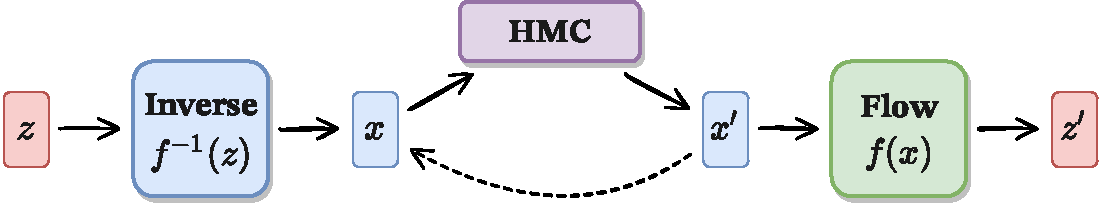
\includegraphics[width=\textwidth]{assets/fthmc.pdf}
    \caption{\label{fig:fthmc}Normalizing flow with inner HMC block.}
\end{figure}
%
\subsection{\label{subsec:hmc}Hamiltonian Monte Carlo (HMC)}
We describe the general procedure of the Hamiltonian Monte Carlo
algorithm~\cite{Betancourt:2017}.
\begin{enumerate}
    \item Introduce \(v \sim \mathcal{N} (0,\mathbb{I}_{n}) \in \mathbb{R}^{n}\)
        and write the joint distribution as
        \begin{equation}
            p(x, v) = p(x) p(v) \propto e^{-S(x)} e^{-\frac{1}{2} v^{T} v}
        \end{equation}
    \item Evolve the joint system \((\dot x, \dot v)\) according to
        Hamilton's equations along \(H=\text{const.}\) using the leapfrog
        integrator:
        \begin{equation}
            \textbf{ (a.)  } \tilde{v} \leftarrow v - \frac{\varepsilon}{2}\partial_{x}S(x)\quad
            \textbf{ (b.)  } x' \leftarrow x + \varepsilon \tilde{v}\quad
            \textbf{ (c.)  } v' \leftarrow \tilde{v} - \frac{\varepsilon}{2}\partial_{x} S(x')
        \end{equation}
    \item Accept or reject the proposal configuration using the
        Metropolis-Hastings test,
        \begin{equation}
            x_{i+1} = \begin{cases}
                x' \text{ with probability } 
                    A(\xi'|\xi) \equiv \min\left\{1, \frac{p(\xi')}{p(\xi)}%
                    \left|\frac{\partial\xi'}{\partial\xi^{T}}\right|\right\}\\
                x \text{ with probability } 1 - A(\xi'|\xi)
            \end{cases}
        \end{equation}
\end{enumerate}


\section{%
    \label{sec:gauge_theory}%
    2D \texorpdfstring{\(U(1)\)}{U(1)} Gauge Theory
}
%
\begin{wrapfigure}{r}{.33\columnwidth}
  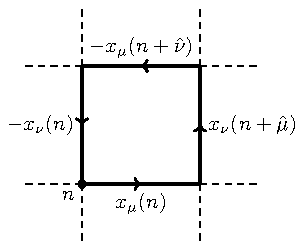
\includegraphics[width=0.33\columnwidth]{assets/plaq.pdf}
  \caption{\label{fig:plaq} Elementary plaquette \(x_{P}\) on the lattice.}
\end{wrapfigure}
%
Let \(U_{\mu}(n) = e^{i x_{\mu}(n)}\in U(1)\), with \(x_{\mu}(n)\in [-\pi,
\pi]\) denote the \emph{link variables}, where \(x_{\mu}(n)\) is a link at the
site \(n\) oriented in the direction \(\hat{\mu}\).
%
We can write our target distribution \(p(x)\) in terms of the Wilson action
\(S(x)\) as
%
\begin{equation}
    p(x)\propto e^{-S(x)},\quad S(x) \equiv \sum_{P} 1 - \cos x_{P}
\end{equation}
%
and \(x_{P} = x_{\mu}(n) + x_{\nu}(n+\hat{\mu}) - x_{\mu}(n+\hat{\nu}) -
x_{\nu}(n)\), as shown in Fig.~\ref{fig:plaq}.
%
For a given lattice configuration, we can define the topological charge
\(Q\in\mathbb{Z}\) as
%
\begin{equation}
    Q = \frac{1}{2\pi}\sum_{P}\mathrm{arg}(x_{P}),
\end{equation}
%
where \(\mathrm{arg}(x_{P})\in[-\pi,\pi]\).
%
\textcolor{blue}{We are interested in how this quantity evolves over a finite length Markov
chain, and in particular, we can define the tunneling rate, \(\delta Q\) as}

\marginpar{\color{red}{Remove references to \(\delta Q\)?}}
%
\begin{equation}
    \delta Q = \sqrt{\left(Q_{i+1} - Q_{i}\right)^{2}}
\end{equation}
%
\textcolor{blue}{where the difference is between subsequent states in the chain.}
%
\textcolor{blue}{This quantity is analogous to the lag-one autocorrelation in the
topological charge.}
%
\section{\label{sec:results}Results}
%
For traditional HMC, we see in Fig~\ref{subfig:q8},\ref{subfig:q16}
that \(Q \simeq 0\) for across all trajectories for both \(8\times 8\) and
\(16\times 16\) lattice volumes.
\marginpar{\textcolor{blue}{Update text}}
%
Conversely, we see in Fig~\ref{subfig:q8},\ref{subfig:q16} that
multiple tunneling events (characterized by \(\delta Q > 0\)) occur for both
\(8 \times 8\) and \(16 \times 16\) volumes.
%
\begin{figure}[htpb]
    \centering
    % \begin{subfigure}[b]{0.49\textwidth}
    %     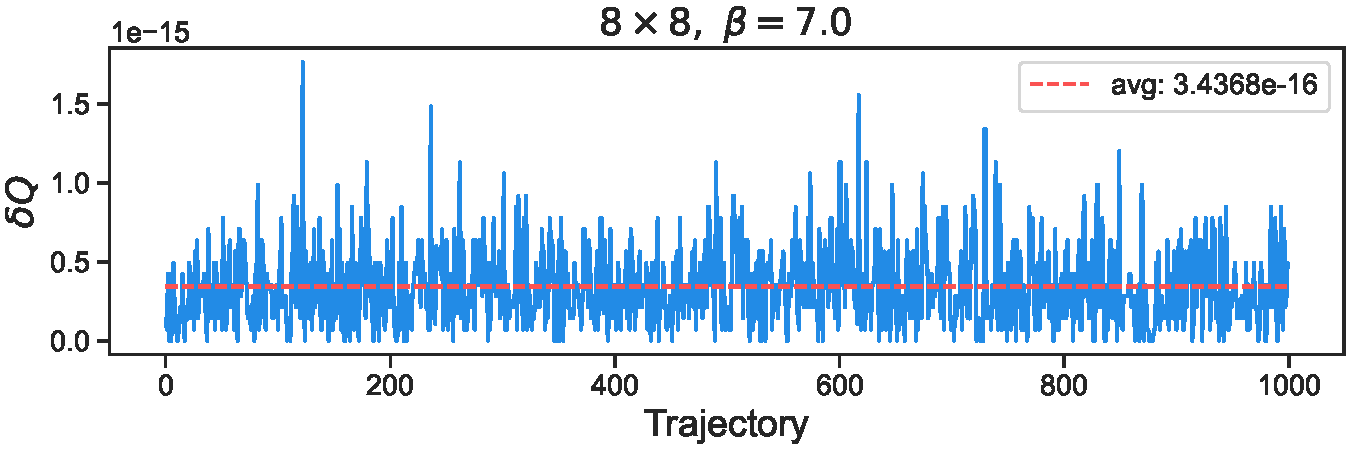
\includegraphics[width=\textwidth]{assets/dqHMC_8x8_beta7.pdf}
    %     \caption{\label{subfig:dqHMC8}HMC, on \(8 \times 8\) lattice at
    %         \(\beta = 7\). Note \(\delta Q \simeq 0\)}
    % \end{subfigure}
    % \hfill
    % -----------------------------------------------
    \begin{subfigure}[b]{\textwidth}
        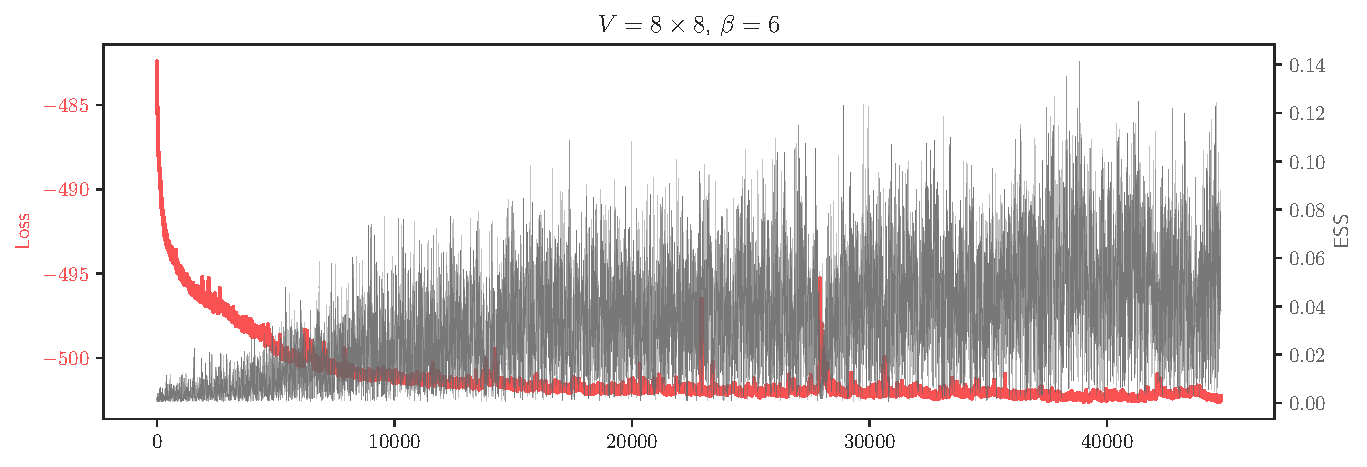
\includegraphics[width=\textwidth]{assets/ess_loss_dkl_train.pdf}
        \caption{\label{subfig:loss}Loss and ESS vs train epoch at \(\beta =
        6\) on \(V = 8\times 8\) lattice.}
    \end{subfigure}
    \begin{subfigure}[b]{\textwidth}
        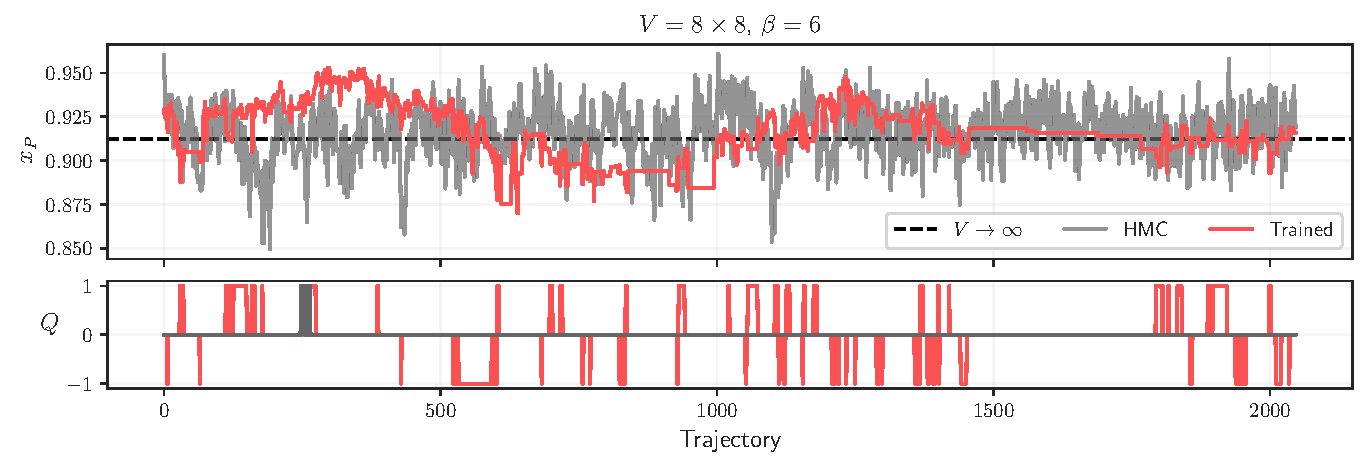
\includegraphics[width=\textwidth]{assets/histories_8x8_beta6.pdf}
        \caption{\label{subfig:q8}\(x_{P}\) and \(Q\) histories for both HMC
            and the trained model, at \(\beta = 6\) with \(V = 8 \times 8\)
        lattice.}
    \end{subfigure}
    \hfill
    \begin{subfigure}[b]{\textwidth}
        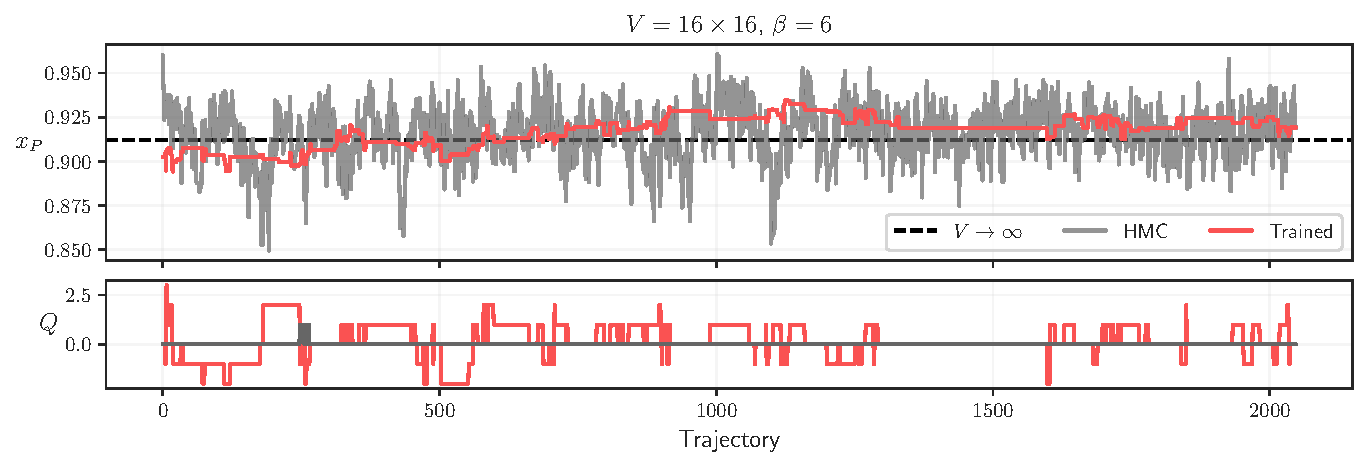
\includegraphics[width=\textwidth]{assets/histories_16x16_beta6_xfr.pdf}
        \caption{\label{subfig:q16}The same model from Fig~\ref{subfig:q8} used
        to generate configurations on \(V = 16\times16\) lattice.}
        % lattice, transferred from model trained on \(8\times8\) lattice. }
    \end{subfigure}
    \caption{\label{fig:histories}}
\end{figure}
%

\textcolor{blue}{NOTE: The HMC data in Fig~\ref{subfig:q16} is incorrectly
reusing the same data from the \(8\times8\) run in Fig~\ref{subfig:q8} (the
Trained data is correct, however). I will update this soon.}

\subsection{\label{subsec:volume_scaling}Volume Scaling}
%
We use gauge equivariant coupling layers that act on plaquettes as the
base layer for our network architecture.
%
As in~\cite{Albergo:2021vyo}, these layers are composed of inner coupling
layers which are implemented as stacks of convolutional layers.
%
One advantage of using convolutional layers is that we can re-use the trained
weights when scaling up to larger lattice volumes.
%
Explicitly, when scaling up the lattice volume we can initialize the weights
of our new network with the previously trained values.
%
This approach has the advantage of requiring minimal retraining effort while
being able to efficiently generate models on large lattice volumes.


% \begin{thebibliography}{99}
\bibliography{main}
\bibliographystyle{plain}
% \bibitem{...}

% \end{thebibliography}

\end{document}
